\documentclass[12pt]{article}
\usepackage{fullpage}
\usepackage{graphicx}
\usepackage{amsthm,amsfonts,amssymb,amsthm}

\theoremstyle{plain}
\newtheorem{thm}{Theorem}
\newtheorem{lem}[thm]{Lemma}
\newtheorem*{cor}{Corollary}

\theoremstyle{definition}
\newtheorem{defn}{Definition}
\newtheorem{exmp}{Example}


\begin{document}

\begin{titlepage}
\title{Computing Mondshein Sequence in Linear Time}
\author{Hemant Saxena}
\date{\today}
\maketitle
\begin{center}
University of Waterloo \\
CS762 - Write Project
\end{center}
\end{titlepage}


\section{Background} \label{sec:background}
We have seen before in lecture notes that canonical ordering is a useful tool for graph drawing, we used it to prove some planar graph properties e.g. Splitting to three trees, Visibility representation.
A quick recall about the canonical ordering: 
\textit{Its a vertex order $v_1,v_2,...,v_n$ of a triangulated planar graph where, $v_1v_2v_n$ is an outer face and all other vertices have at least two predecessors and at least one successor.}
Canonical order exist for any 3-connected planar graph \cite{kant}, in these notes we extend the canonical ordering for non-planar graphs and make them applicable for an arbitrary 3-connected graphs.

The idea of canonical orderings was given much before, in 1971 by Lee F. Mondshein at M.I.T. in his PhD-thesis \cite{mond}.
Mondshein proposed a sequence that generalizes canonical orderings to non-planar graphs.
Mondshein's sequence was later, in 1988 were independently found by Cheriyan and Maheshwari \cite{cheriyan} under the concept of \textit{non-separating ear decompositions}.
Complexity of calculating Mondshein sequences, is an intriguing question.
Mondshein himself gave an algorithm with running time of $O(m^2)$.
Cheriyan in his work achieved a running time of $O(nm)$ by using Tutte's theorem that proves the existence of non-separating cycles in 3-connected graphs \cite{tutte1963draw}.
The challenge of achieving a sub-quadratic time for calculating Mondshein sequences was still open.
The work by Jens M. Schmidt \cite{Schmidt13a} presents the first algorithm that computes a Mondshein sequence in $O(m)$ time and space, and this will be the major focus of these notes.
The motivation for computing Mondshein sequence in sub-quadratic time stems around three main applications of it, that can now be solved in linear-time.
First, computing three independent spanning trees in a 3-connected graph in linear time.
Second, linear time processing of the output-sensitive data structure by Di Battista et. al. \cite{Battista} that reports three internally disjoint paths between any given vertex pair.
Third, a simple linear-time planarity testing.


\section{Ear Decomposition and Mondshein sequence} \label{sec:earMond}
This section will give an overview of ear-decomposition and Mondshein-sequences.
\subsection{Ear Decomposition}
\begin{defn}\label{def:eardecomp}
An \textit{ear decomposition} of a 2-connected graph $G=(V,E)$ is a decomposition $G = (P_0, P_1,... P_K)$ that partitions E,
where $P_0$  is a cycle and $P_i, 1 \leq i \leq K$ is a path with only its two distinct end vertices in common with $(P_0 \cup P_1 \cup ... \cup P_{i-1})$. 
Each $P_i$ is called an \textit{ear}.
\end{defn}

\begin{figure}
    \centering
    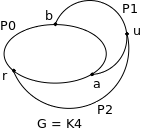
\includegraphics[scale=0.6]{earDecomp.png} \\
    \caption{An example of ear decomposition of a $K_4$ containing 3 ears.}
    \label{fig:earDecomp}
\end{figure}

Now we will define some terms associated with an ear decomposition.
An \textit{ear} is called \textit{short} if it is an edge and \textit{long} otherwise.
For any $i$, let $G_i = (P_0 \cup P_1 \cup ... \cup P_{i})$ and $\overline{V_i} := V - V(G_i)$, and $\overline{G_i}$ is a graph induced by $\overline{V_i}$.
Note that, $\overline{G_i}$ does not necessarily contain all edges in $E - E(G_i)$, there can be short ears which have both the end points in $G_i$.
For a path $P$ and two of its vertices $x$ and $y$, $P[x,y]$ be the sub-path in P from $x$ to $y$.
A path with endpoints $v$ and $w$ is called a \textit{vw-path}.
A vertex $x$ in a \textit{vw-path} is called an \textit{inner vertex} if $x \notin \{v,w\}$.
For simplicity we assume that every vertex in $P_0$ is an inner vertex.
\textit{inner(P)} denotes a set of inner vertices of an ear P.
For an edge $e \in G$, $birth(e)$ is the index $i$ where $e$ is born, i.e. $i$ such that $P_i$ contains $e$.
Similarly, for a vertex $v \in G$, $birth(v)$ is the index $i$ of the first path $P_i$ that contains $v$, 
in other words, $P_{birth(v)}$ is the ear containing $v$ as an inner vertex.

\begin{defn}\label{def:nonseperating}
Let $D = (P_0, P_1,... P_K)$ be an ear decomposition of G.
D is defined as a \textit{non-separating} ear decomposition if, for all $i, 0 \leq i \leq k$, $\overline{G_i}$ is connected  
and each internal vertex of ear $P_i$ has a neighbor in $\overline{G_i}$.
\end{defn}

We will now see how canonical ordering for a plane graph can be expressed using a non-separating ear decomposition.

\begin{defn}\label{def:canonical}
Canonical ordering (another definition).
Let G be a 3-connected plane graph having edges $v_1v_2$ and $v_2v_n$ on its outer face.
A \textit{canonical ordering} with respect to $v_1v_2$ and $v_2v_n$ is an ear decomposition D of G such that:
\begin{enumerate}
\item $v_1v_2 \in P_0$,
\item $P_{birth(v_n)}$ is the last long ear, that contains $v_n$ as its only inner vertex and does not contain $v_2v_n$, and
\item D is non-separating.
\end{enumerate}
\end{defn}

\textit{How is the above definition similar to old definition (Def. 8.1 in lecture notes) of canonical ordering?}
Recall, old definition (Def 8.1 in lecture notes) also had $v_1,v_2,v_n$ fixed on the outer triangular face.
Edge $v_1v_2$ was first fixed on the outer face and we incrementally formed G by adding $v_{k+1}$ to $G_k$ at each step.
Vertex $v_{k+1}$ was adjacent to two or more outer-face vertices of $G_k$, in other words $G_k$ was connected to $\overline{G_k}$, hence property 3 makes sense.
Vertex $v_n$ was added at last, one can imagine arc $v_1v_nv_i$, $i \notin \{1,2,n\}$ as a last long ear where $v_n$ is an inner vertex.
The difference (between Def \ref {def:canonical} and Def 8.1 in lecture notes) lies in property 2, remember that in lecture we saw canonical ordering for a triangulated graphs, 
but Def. \ref{def:canonical} is for any 3-connected graph, therefore vertex $v_n$ should have degree at least three.
Hence, long ear $P_{birth(v_n)}$ cannot contain $v_2v_n$; $v_2v_n$ should be a short ear.
It is also evident that adding vertex $v_3$ forms a cycle $v_1v_2v_3$, think of it as $P_0$ in the above definition.


\subsection{Mondshein sequence}
Now we will see how can Definition \ref{def:canonical} be extended for non-planar graphs.
Notice that Definition \ref{def:canonical} uses planarity only at one place: we assumed edges $v_1v_2$ and $v_2v_n$ are on the outer face.
By dropping this assumption we can generalize Definition \ref{def:canonical} for non-planar graphs, all we need is that $v_1v_2$ and $v_2v_n$ should be edges in graph G.

In 1971, Mondshein used a similar definition to define a $(2,1)-sequence$ [\cite{mond} Def. 2.2.1], but it was in the notation of a special vertex ordering.
For conciseness, we will stick to the ear-decomposition based definition in these notes, which is similar to the one given by Cheriyan \cite{cheriyan}.

\begin{defn}\label{def:mond}
(\cite{mond}, \cite{cheriyan}). Let G be a graph with an edge $v_2v_n$. A \textit{Mondshein sequence avoiding $v_2v_n$} is an ear decomposition D of G such that:
\begin{enumerate}
\item $v_2 \in P_0$
\item $P_{birth(v_n)}$ is the last long ear, that contains $v_n$ as its only inner vertex and does not contain $v_2v_n$, and
\item D is non-separating.
\end{enumerate}
\end{defn}

In other words the edge $v_2v_n$ is added last in D as a short ear, right after the last long ear $P_{birth(v_n)}$ has been added, and as a direct consequence of property (2) and (3), 
G must have a minimum degree 3 to have a Mondshein sequence.
This has also been explained after Def. \ref{def:canonical}.
Moreover, Mondshein in his thesis \cite{mond} proved that every 3-connected graph has a Mondshein sequence.
\textit{If D satisfies property (1) and (2) it is said to avoid $v_2v_n$.}


\section{Computing a Mondshein Sequence} \label{sec:computingMond}
As mentioned in Section \ref{sec:background}, Mondshein himself gave an $O(m^2)$ algorithm to compute his sequence \cite{mond}, later Cheriyan gave an $O(mn)$ time algorithm \cite{cheriyan}.
The main focus of these notes is the linear time algorithm proposed by Schmidt \cite{Schmidt13a} to compute a Mondshein sequence.
At the core of Schimdt's algorithm lies a classical construction of 3-connected graphs proposed by Barnette and Grunbaum \cite{bg} and Tutte [\cite{tutteConnectivity}, Thms. 12.64 and 12.65].
Before describing the Schimidt's algorithm, we will first see what are \textit{BG-Operations}.

\subsection{BG-Operations}

\begin{defn} \label{def:bg}
The following operations on simple graphs are BG-operations (See Fig \ref{fig:bg}):
\begin{enumerate}
\item \textit{vertex-vertex-addition}: Add an edge between two distinct non-adjacent vertices.
\item \textit{edge-vertex-addition}: Subdivide an edge $ab$, $a \ne b$, by a vertex $v$ and add an edge $vw$ where $w \notin \{a,b\}$.
\item \textit{edge-edge-addition}: Subdivide two distinct edges by vertices $v$ and $w$, respectively, and add the edge $vw$.
\end{enumerate}
\end{defn}

\begin{figure}
    \centering
    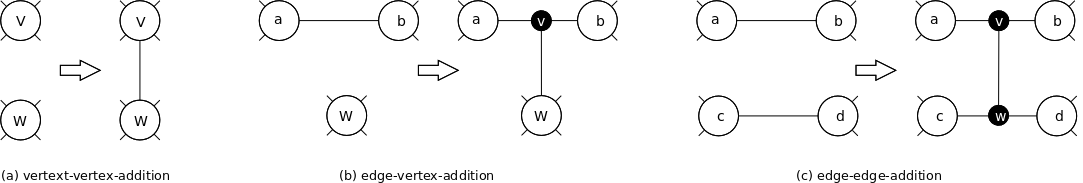
\includegraphics[scale=0.3]{bg.png} \\
    \caption{BG Operations as described in Def. \ref{def:bg}.}
    \label{fig:bg}
\end{figure}

Barnette and Grunbaum, and Tutte also gave the following Theorem:

\begin{thm} \label{thm:k4bg}
(\cite{bg}, \cite{tutteConnectivity}). A graph is 3-connected if and only if it can be constructed from $K_4$ using the \textit{BG-operations}.
\end{thm}

It can be seen from Theorem \ref{thm:k4bg} that applying BG-operation on 3-connected graphs keeps them simple and 3-connected.
Figure \ref{fig:bgEg} gives an example of obtaining $K_5$ from $K_4$ using BG-operations.
A sequence of BG-operations that construct G from $K_4$ is known as \textit{BG-sequence}.
Theorem 6 and 52 in \cite{bgLinear} shows that BG-sequence of a 3-connected graph can be computed in time $O(m)$.
\begin{figure}
    \centering 
    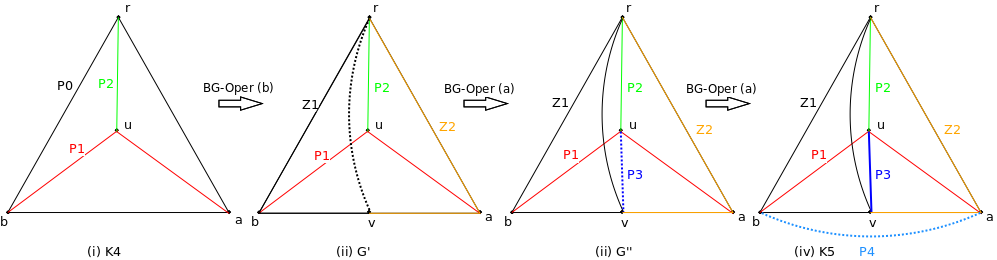
\includegraphics[scale=0.27]{bgEg.png} \\ 
    \caption{Obtaining $K_5$ from $K_4$ using BG-operations. Pi and Zi shows the ear decomposition. Dotted line denotes the newly added edge.}
    \label{fig:bgEg}
\end{figure}



\subsection{Algorithm}
We will first give an overview of the algorithm and later go into the detailed cases.
The algorithm starts with computing a Mondshein sequence of $K_4$, which is easy.
Then using Theorem \ref{thm:k4bg} we construct our G in a step by step manner from $K_4$, this can be done in linear time, as BG-sequence can be computed in linear time.
Our claim is that, each BG-operation in the BG-sequence of $G'$ to G, modifies the Mondshein sequence in a well defined way given by Lemma \ref{lem:cases}.
In other words there are finite number of cases to which each BG-operation can be mapped while transforming G' to G, and each of those cases have finite number of additions to the Mondshein sequence of G'.
This gives us a Mondshein sequence of G from the Mondshein sequence of G'.

\begin{exmp}
For example, Figure \ref{fig:bgEg} explains the changes in Mondshein sequence when obtaining $K_5$ from $K_4$.
Mondshein sequence of $K_4$ is [P0, P1, P2] (follow the color coding).
After applying $BG-Oper(b)$ on $K_4$, which maps to case 2aiii of Lemma \ref{lem:cases} (defined later), we get G' and mondshein sequence is [Z1, Z2, P1, P2].
After $BG-Oper(a)$ on G', which maps to case 1 of Lemma \ref{lem:cases}, we get G'' and Mondshein sequence is [Z1, Z2, P1, P2, P3].
In the final operation $BG-Oper(a)$ which again maps to case 1 of Lemma \ref{lem:cases}, we get $K_5$ and final Mondshein sequence is [Z1, Z2, P1, P2, P3, P4].
\end{exmp}

Now we will define some notations for describing the modifications.
Let $\Gamma$ be a single BG-operation, that adds edge $vw$, if applicable, as described in Def. \ref{def:bg}.
Whenever we consider edges $ab$ and $cd$, without loss of generality (w.l.o.g) we assume that $birth(a) \leq birth(b), birth(c) \leq birth(d)$ and $birth(d) \leq birth(b)$.
Let set $S \subseteq \{av,vb,vw,cw,wd\}$ be the set of new edges added after operation $\Gamma$, see figure \ref{fig:bg}.

The following Lemma describes a detailed scheme of modifying Mondshein sequence for each possible scenario of applying $\Gamma$ on G.

\begin{lem} \label{lem:cases}
There is a Mondshein sequence $D' = (P_0',P_1',...,P_{k+1}')$ of G' avoiding ru (respectively, rv or rw if applicable) that can be obtained from $D = (P_0,P_1,...,P_k)$ of G by performing the following four modifications:

\begin{enumerate}
\item[M1)] replacing the long ear $P_{birth(b)}$ with $P_{b1}', P_{b2}', P_{b3}'$ in order and if applicable. Each $P_{bi}'$ consists of edges in $P_{birth(b)} \cup S$.
\item[M2)] if $P_{birth(cd)}$ is a long ear and $birth(d) < birth(b)$, subdivide $cd$ with $w$ and replace $P_{birth(cd)}$ with the long ear $P_{birth(cwd)}'$.
\item[M3)] if $P_{birth(ab)}$ is short, delete or replace $P_{birth(ab)}$ with an edge in \{av,vb,vw\}; if $P_{birth(cd)}$ is short, delete or replace $P_{birth(cd)}$ with an edge in \{cw,wd\}.
\item[M4)] adding vw as new last ear, if applicable.
\end{enumerate}

In particular, each $\Gamma$ lies in one of the following cases and defines the construction of D' from D, also shown in Fig. \ref{fig:algoCases} :
\begin{enumerate}
\item $\Gamma$ is a vertex-vertex-addition: use M4.
\item $\Gamma$ is an edge-vertex-addition: This case will depend whether b is an inner vertex or not
	\begin{enumerate}
	\item w.l.o.g. birth(b) = birth(ab), i.e. b is an inner-vertex.
	Let a' and b' be the endpoints of $P_{birth(b)}$ such that a' is closer to a than to b.
	Let $P_{avb}'$ be the path obtained by subdividing ab in $P_{birth(b)}$ with v.
	This will have three cases depending upon w's position:
		\begin{enumerate}
		\item $w \notin G_{birth(b)}$ i.e. $birth(w) > birth(b)$ \\
		Obtain $P_{avb}'$ from $P_{birth(b)}$ and add ear vw at the end.
		\item $w \in G_{birth(b)} - P_{birth(b)}$ i.e. $birth(w) < birth(b)$ and $w \notin \{a',b'\}$ \\
		Obtain $P_{avb}'$ from $P_{birth(b)}$ and replace $P_{birth(b)}$ with $Z_1 = a'w-path$ and $Z_2 = vb'-path$ in this order to obtain D'.
		\item $w \in P_{birth(b)}$ i.e. $birth(w) = birth(b)$ or $w \in \{a',b'\}$ \\
		Obtain $Z = P_{avb}'$ from $P_{birth(b)}$. Let $Z_2 = vw-path$, $Z_1 = Z - Z_2 + vw$.
		(If $P_{birth(b)}$ is $P_0$ then there will be two vw-path, choose the one not containing r as an inner vertex.)
		Get D' by replacing $P_{birth(b)}$ with $Z_1$ and $Z_2$ in this order, (from now on we will call this process as applying $M1(Z_1,Z_2,\o)$, with $P_{b1}'=Z_1, P_{b2}'=Z_2, P_{b3}' = \o $.)
		\end{enumerate}
	\item w.l.o.g. birth(b) $<$ birth(ab) and $P_{birth(ab)} = ab$, i.e. b is not an inner vertex. Note that ear $P_{birth(ab)}$ cannot be long as a and b have to be born before ab.
	Again three cases depending upon w's position:
		\begin{enumerate}
		\item $birth(w) > birth(b)$ \\
		Replace $P_{birth(ab)} = ab$ with ear $av \cup vb$ and add ear ear vw at the end.
		\item $birth(w) < birth(b)$: cases depending upon a's relation with b.
			\begin{enumerate}
			\item $birth(a) < birth(b)$ \\
			If ab = ru, add new ear $wv \cup vu$ directly after $P_{birth(u)}$ and replace $P_{birth(ru)} = ru$ with rv.
			If ab $\neq$ ru, add new ear $av \cup vw$ directly after $P_{birth(b)-1}$ and replace $P_{birth(ab)} = ab$ with vb.
			\item $birth(a) = birth(b)$ \\
			Let $Z_1 = av \cup vw \cup P_{birth(b)}[a',a]$ and $Z_2 = P_{birth(b)}[a,b']$. Apply $M1(Z_1,Z_2,\o)$ and replace $P_{birth(ab)} = ab$ with vb.
			\end{enumerate}
		\item $birth(w) = birth(b)$ \\
		If $birth(a) = birth(b) > 0$, let a' and b' be the endpoints of $P_{birth(b)}$ such that a' is closer to a than to b.
		Cases depending upon a's relation with b:
			\begin{enumerate}
			\item $birth(a) = birth(b) > 0$ and w lies strictly between either a and a' or b and b' in $P_{birth(b)}$, (say w.l.o.g. between b and b') \\
			Let $Z_1 = av \cup vw \cup P_{birth(b)}[a',a] \cup P_{birth(b)}[w,b'] $ and $Z_2 = P_{birth(b)}[a,w]$.
			Apply $M1(Z_1,Z_2,\o)$ and replace $P_{birth(ab)} = ab$ with vb.
			\item $birth(a) = birth(b) > 0$ and w lies strictly between a and b in $P_{birth(b)}$.\\
			Let $Z_1 = av \cup vb \cup P_{birth(b)}[a',a] \cup P_{birth(b)}[b,b'] $ and $Z_2 = P_{birth(b)}[a,b]$.
			Apply $M1(Z_1,Z_2,\o)$ and replace $P_{birth(ab)} = ab$ with vw.
			\item $birth(a) = birth(b) = 0$ \\
			In this case we are at $P_0$, consider $P_0 = P_{ab} \cup P_{bw} \cup P_{wa}$, one of these path must contain r, say $P_{ab}$.
			Let Z be the union of remaining two paths, $Z = P_{bw} \cup P_{wa}$.
			Let $P_0'$ be the cycle 'arbva', and $Z_2 = Z$ added directly after $P_0'$, and replacing $P_{birth(ab)} = ab$ with vw, i.e. connect v to vertex $j \in \{a,b,w\}$ that is not an endpoint of Z.
			\item $birth(a) < birth(b)$ \\
			Let b' and b'' be the two endpoints of $P_{birth(b)}$ such that b' is closer to w than to b.
			If $b' \neq a$, $Z_1 = av \cup vw \cup P_{birth(b)}[w,b']$ and $Z_2 = P_{birth(b)}[w,b'']$.
			If $b' = a$,  $Z_1 = av \cup vb \cup P_{birth(b)}[b',b'']$ and $Z_2 = P_{birth(b)}[b,b']$.
			Apply $M1(Z_1,Z_2,\o)$ and replace $P_{birth(ab)} = ab$ with vw.
			\end{enumerate}
		\end{enumerate}
	\end{enumerate}
\item $\Gamma$ is an edge-edge-addition: It will again depend whether b is an inner vertex or not. 
(Due to space constraints we will only see 2 of the 13 cases described in \cite{Schmidt13a}.)
	\begin{enumerate}
	\item[3aiA)] $birth(b)=birth(ab)$ (inner vertex), $birth(d) < birth(b)$ and $birth(cd) < birth(b)$.\\
	Let a' and b' be the endpoints of $P_{birth(b)}$ such that a' is closer to a than to b.
	Subdivide ab with v. Then $Z_1 =  P_{birth(b)}[a',v] \cup vw$ and $Z_2 =  P_{birth(b)}[v,b']$.
	$P_{birth(cd)}$ can be short or long. If $P_{birth(cd)} = cd$ (i.e. short), delete $P_{birth(cd)}$ and apply $M1(cw \cup wd, Z_1, Z_2)$.
	If $P_{birth(cd)}$ is long, apply M2 and $M1(Z_1, Z_2, \o)$.
	\item[3biiC)] birth(b) $<$ birth(ab) and $P_{birth(ab)} = ab$, $birth(d) = birth(b)$, $birth(a) < birth(b)$ and $C \notin P_{birth(b)}$. \\
	Then $P_{birth(cd)} = cd$, have to be a short ear, because $C \notin P_{birth(b)}$, $birth(d) = birth(b)$ and $birth(c) < birth(d)$.
	Let b' and b'' be the two endpoints of $P_{birth(b)}$ such that b' is closer to d than to b on $P_{birth(b)}$ (a may be in $\{b',b'',c\}$).
	There can be cases where b=d, and b=d and $ru\in \{ab,cd\}$, but due to space constraint we will not go into their details.
	Consider $b \neq d$, $Z_1 =  P_{birth(b)}[d,b'] \cup cw \cup wd$, $Z_2 = av \cup vw$ and $Z_3 =  P_{birth(b)}[d,b'']$.
	Apply $M1(Z_1,Z_2,Z_3)$, delete $P_{birth(cd)} = cd$ and replace $P_{birth(ab)} = ab$ with vb.
	\end{enumerate}
\end{enumerate}
\end{lem}

\begin{figure}
    \centering
    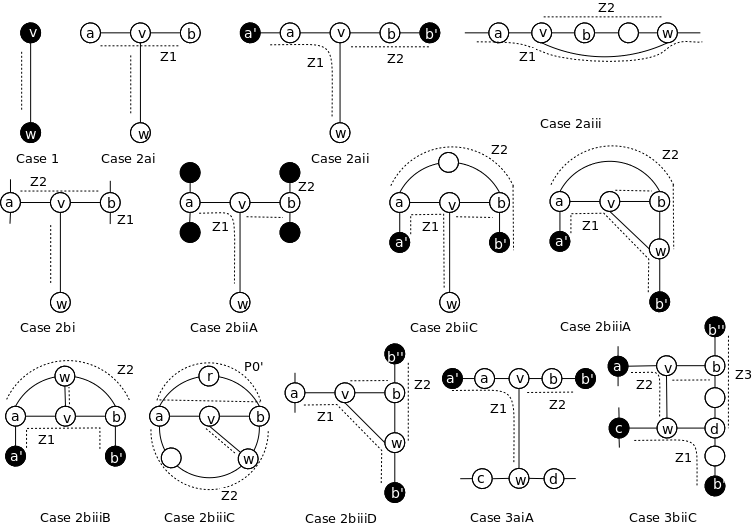
\includegraphics[scale=0.3]{algoCases.png} \\
    \caption{Case 1, 2 and 3 of the Lemma \ref{lem:cases}. Black vertices are the endpoints of the ears that are contained in $G_{birth(b)}$. Dashed paths are part of the ears in D'.}
    \label{fig:algoCases}
\end{figure}



\section{Proof of Lemma \ref{lem:cases}} \label{sec:proof}
\textbf{Completeness} - We will first prove that Lemma \ref{lem:cases} covers all the possible cases of BG-operations.
Case (1) is simple and cannot have further subdivisions in the main case.
Case (2), is an edge-vertex-operation.
W.l.o.g we can choose either vertex $a$ or $b$ to look all possible relations with $birth(ab)$, say $b$.
Observe, only two possibilities, either $b$ will be an inner vertex of $P_{birth(ab)}$ or not, hence $birth(b) < birth(ab)$ or $birth(b) = birth(ab)$.
Third vertex in Case (2) is $w$, it can either be in $P_{birth(b)}$ or in $G_{birth(b)} - P_{birth(b)}$ or in $\overline{G_{birth(b)}}$, and hence three cases under (2a) and (2b).
See \cite{Schmidt13a} for completeness of case (3).

\medskip
\textbf{D' is an ear decomposition} - As the newly added ears in all the cases are paths, it is sufficient to show that only the first ear, $P_0'$ in D' is a cycle.
The only cases which can modify $P_0$ are (2ai), (2aiii), (2bi), (2biiic), and some cases in (3) (see \cite{Schmidt13a}).
All of these cases can subdivide an edge in $P_0$ by a new vertex and replace a path in $P_0$ with a shorter one having the same endpoints.
This will still maintain a cycle in D'.
Hence D' is an ear decomposition.

\medskip
\textbf{D' avoids $ru$ ($rv$ or $rw$ if applicable) } - Recall Def \ref{def:mond}, to prove this we need show that D' satisfy conditions (1) and (2) of Def. \ref{def:mond}.
To prove condition (1), it is sufficient to consider cases where $P_0$ is different from $P_0'$, i.e. cases (2aiii), (2biiic) and some in case (3).
In all the cases, a path of $P_0$ that does not contain $r$ has been modified, therefore $r \in P_0'$ also.
This shows condition (1) is satisfied.

To prove condition (2), first consider the vertex-vertex-addition: only a short ear is added at the end, hence satisfied.
Now consider a edge-vertex-addition, first consider the case where $v$ does not subdivide $ru$.
$P_{birth(u)}$ is the last long ear in D, therefore $birth(u) \geq birth(b)$.
If $birth(u) > birth(b)$, that means change is in $P_{birth(b)}$ and $P_{birth(u)}$ is unchanged and is still a last long ear in D'.
Thus, condition (2) satisfied for this case.

If $birth(u) = birth(b)$, and as $P_{birth(b)}$ has $b$ as inner vertex, it is long; this implies $b=u$ as $u$ is the only inner vertex of $P_{birth(u)}$.
Now it will depend if $a \in P_{birth(b)}$, $a$ must be a neighbor of the inner vertex $b=u$ and $birth(ab) = birth(b)$ follows and also $w \in G_{birth(b)}$, because we are at the last ear.
This means we are in case (2aii) or (2aiii).
In both these cases $Z_2$ (the last long ear) contains exactly $b=u$ as the inner vertex and does not contain $ru$, hence condition (2) satisfied.
If $a \notin P_{birth(b)}$, $birth(a) < birth(b) < birth(ab)$ and again $w \in G_{birth(b)}$, therefore we are in case (2biiA) with $a \neq r$.
See that in this case $P_{birth(b)}$ remains unchanged and no long ear is added after $P_{birth(b)}$, hence condition (2) satisfied.

Now lets assume that $v$ subdivides $ru$.
This mean $a=r$ and $b=u$ with $birth(a) < birth(b)$, as $r \in P_0$ and $u \notin P_0$.
Also, as D satisfies condition (2), it cannot have $ab=ru$ in its last long hear, hence, is itself a short ear.
Also $w \in G_{birth(b)}$, hence we are in case (2biiA) with $ab = ru$.
In this ear $wv \cup vb$ is added as last long ear and $av$ is the new avoided edge of D', hence condition (2) satisfied.

See \cite{Schmidt13a} for edge-edge-addition correctness.

\medskip
\textbf{D' is non-separating} - Consider $D' = (P_0', P_1', ... ,P_{k+1}')$ and let $z$ be any inner vertex of $P_i'$.
It suffices to prove that $z$ has a neighbor in $\overline{G_i'} \neq \o$.
First consider the vertex-vertex-addition: it only adds a short ear at the end, hence the configuration of all long ears remains identical in D and D'.
Given that D is non-separating, D' is also non-separating.

Now consider a edge-vertex-addition.
We will see an overview of the proof, due to space constraints.
Observe that $z=v$ is the only new inner vertex possible in D', compared to D.
It is sufficient to show that $z=v$ has a neighbor in $\overline{G_i'}$.
Table \ref{tab:neighbors} shows the neighbors of $z=v$ in $\overline{G_i'}$ for all the sub-cases in case (2).


\begin{table} \label{tab:neighbors}
  \centering  
  \resizebox{\linewidth}{!}{
    \begin{tabular}{|c|c|c|c|c|c|c|c|c|c|c|}  \hline
         & (2ai) & (2aii) & (2aiii) & (2bi) & (2biiA) & (2biiB) & (2biiiA) & (2biiiB) & (2biiiC) & (2biiiD)	\\ \hline
	Neighbor of v & w & b & a or b & w & b & b & a or b & w & $inner(Z) \cap \{a,b,w\}$ & b or w \\ \hline
    \end{tabular}}
    \caption{Neighbors of $v \in inner(P_i')$ in $\overline{G_i'}$}
  \end{table}


\medskip

This ends the proof of Lemma \ref{lem:cases}.
The paper \cite{Schmidt13a} presents the Case (3) and its proof in more detail, and also presents 3 applications which can now be solved in linear time, because Mondshein sequence can be calculated in linear time. Due to space constraints we conclude these notes here.


\bibliographystyle{abbrv}
\bibliography{project}

\end{document}
